\documentclass{beamer}

% --- 包设置 ---
\usepackage{ctex} % 提供中文支持
\usepackage{amsmath} % 用于数学公式
\usepackage{graphicx}
% --- 主题与颜色 ---
\usetheme{Madrid}
\usecolortheme{default}
\setbeamertemplate{navigation symbols}{} % 隐藏导航条

% --- 文稿信息 ---
\title{节流过程的原理及其关键应用}
\author{陈嗣杰}
\institute{课程:热力学与统计物理}
\date{2025.9.22}


\begin{document}

% --- 标题页 ---
\begin{frame}
  \titlepage
\end{frame}

% --- 目录页 ---
\begin{frame}
  \frametitle{目录}
  \tableofcontents
\end{frame}


% --- 第一部分:引言与基本原理 ---
\section{引言与基本原理}

\begin{frame}
  \frametitle{什么是节流过程?}
  \begin{itemize}
    \item<1-> \textbf{宏观定义:} 流体在\alert{绝热}条件下,流经一个阀门、多孔塞或其他阻碍物,导致其\alert{压强显著降低}的过程。
    \item<2-> \textbf{热力学分析:}
    \begin{itemize}
      \item 考虑一个稳定流动系统,根据热力学第一定律的推广形式:
      $h_1 + \frac{v_1^2}{2} + gz_1 + q = h_2 + \frac{v_2^2}{2} + gz_2 + w_s$
      \item 在节流过程中:
      \begin{itemize}
          \item 绝热:$q=0$
          \item 不做轴功:$w_s=0$
          \item 宏观动能与势能变化通常可忽略:$\Delta E_k \approx 0, \Delta E_p \approx 0$
      \end{itemize}
    \end{itemize}
    \item<3-> \textbf{核心结论:\alert{焓守恒 ($h_1 \approx h_2$)}}。节流过程是一个\alert{等焓}过程。
    
  \end{itemize}
\end{frame}

\begin{frame}
  \frametitle{焦耳-汤姆孙效应 (Joule-Thomson Effect)}
  \begin{columns}[T]
    \begin{column}{0.6\textwidth}
      \begin{itemize}
        \item \textbf{现象:} 节流过程中,实际气体的\alert{温度会发生变化}。
        \vfill
        \item \textbf{焦耳-汤姆孙系数 ($\mu_{JT}$):}
        \begin{itemize}
          \item 定义式:$\mu_{JT} = \left(\frac{\partial T}{\partial P}\right)_H$
          \item $\mu_{JT} > 0$:\alert{节流致冷}。应用最广泛。
          \item $\mu_{JT} < 0$:节流致热。
          \item $\mu_{JT} = 0$:温度不变,对应“转化点”。
        \end{itemize}
        \vfill
        \item \textbf{注意:} 对于\alert{理想气体},由于分子间没有相互作用力,焓只是温度的函数,因此节流过程温度不变,$\mu_{JT} = 0$。
      \end{itemize}
    \end{column}

    \begin{column}{0.4\textwidth}
      \begin{figure}
       \centering
       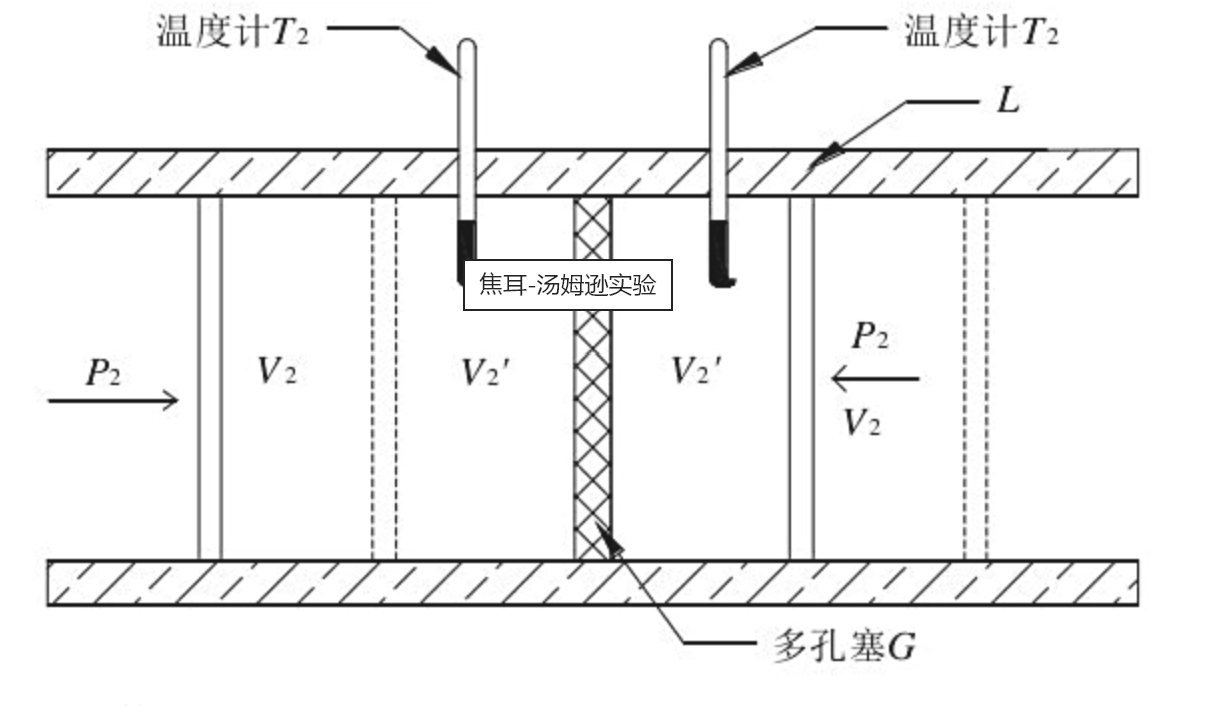
\includegraphics[width=5cm]{image.png}
       \caption{节流过程示意图}
       \end{figure}
    \end{column}
  \end{columns}
\end{frame}

\begin{frame}
    \frametitle{J-T效应的微观解释}
    \begin{itemize}
        \item \textbf{根源:} 实际气体分子间的\alert{相互作用力}和\alert{分子自身体积}。
        \vfill
        \item \textbf{过程分析:} 气体节流膨胀时,分子平均间距增大。
        \begin{itemize}
            \item<2-> \textbf{克服引力做功:} 当分子间距在\alert{引力}起主导作用的范围内,膨胀时分子需要克服引力做功。这部分功消耗了气体内能,导致分子平均动能下降,宏观上表现为\alert{温度降低} ($\mu_{JT}>0$)。
            \vfill
            \item<3-> \textbf{斥力作用减弱:} 当气体被高度压缩,分子间距很小,\alert{斥力}起主导作用。膨胀使得斥力迅速减弱,分子的斥力势能转化为动能,宏观上表现为\alert{温度升高} ($\mu_{JT}<0$)。
        \end{itemize}
        \vfill
        \item<4-> \textbf{结论:} J-T效应的致冷或致热,取决于气体所处状态下,分子间\alert{引力与斥力的相对强弱}。
    \end{itemize}
\end{frame}

\begin{frame}
    \frametitle{转化温度与致冷条件}
    \begin{itemize}
        \item \textbf{转化曲线 (Inversion Curve):} 在P-T图上,所有$\mu_{JT}=0$的点连接成的曲线。
        \begin{itemize}
            \item 曲线内部区域:$\mu_{JT} > 0$,节流致冷。
            \item 曲线外部区域:$\mu_{JT} < 0$,节流致热。
        \end{itemize}
        \vfill
        \item \textbf{最高转化温度:} 转化曲线与T轴的交点。只有当气体的初始温度\alert{低于其最高转化温度}时,才有可能通过节流实现降温。
        \vfill
        \item \textbf{重要实例:}
        \begin{itemize}
            \item \textbf{氮气、氧气、氩气:} 最高转化温度远高于室温,在室温下可以直接通过节流进行液化。
            \item \textbf{\alert{氢气} (T$_{max}$ $\approx$ 205 K) 和 \alert{氦气} (T$_{max}$ $\approx$ 43 K):} 最高转化温度很低,在室温下节流会\alert{升温}。因此,它们在节流前必须被\alert{预冷}到其最高转化温度以下。
        \end{itemize}
    \end{itemize}
\end{frame}

% --- 第二部分:核心应用领域 ---
\section{核心应用领域}

\begin{frame}
  \frametitle{应用一:制冷与空调技术}
    \begin{itemize}
        \item \textbf{核心地位:} 节流是\alert{蒸气压缩制冷循环}不可或缺的一环,起着\alert{降压降温}的关键作用。
        \vfill
        \item \textbf{四大过程:}
        \begin{enumerate}
            \item \textbf{压缩 (Compression):} 压缩机做功,将低温低压制冷剂蒸气压缩成高温高压蒸气。
            \item \textbf{冷凝 (Condensation):} 高温高压蒸气在室外冷凝器中向环境放热,变为高压液体。
            \item \textbf{\alert{节流 (Throttling)}:} 高压液体流经\alert{膨胀阀}或\alert{毛细管},压强和温度骤降,变为低温低压的液汽混合物。
            \item \textbf{蒸发 (Evaporation):} 低温低压制冷剂在室内蒸发器中吸收热量而汽化,实现制冷。
        \end{enumerate}
        \vfill
        \item \textbf{应用实例:} 家用冰箱、空调、汽车空调、冷库、热泵等。
    \end{itemize}
\end{frame}

\begin{frame}
    \frametitle{详解:P-h图中的制冷循环}
    \begin{columns}
        \begin{column}{0.5\textwidth}
           \begin{figure}
             \centering
             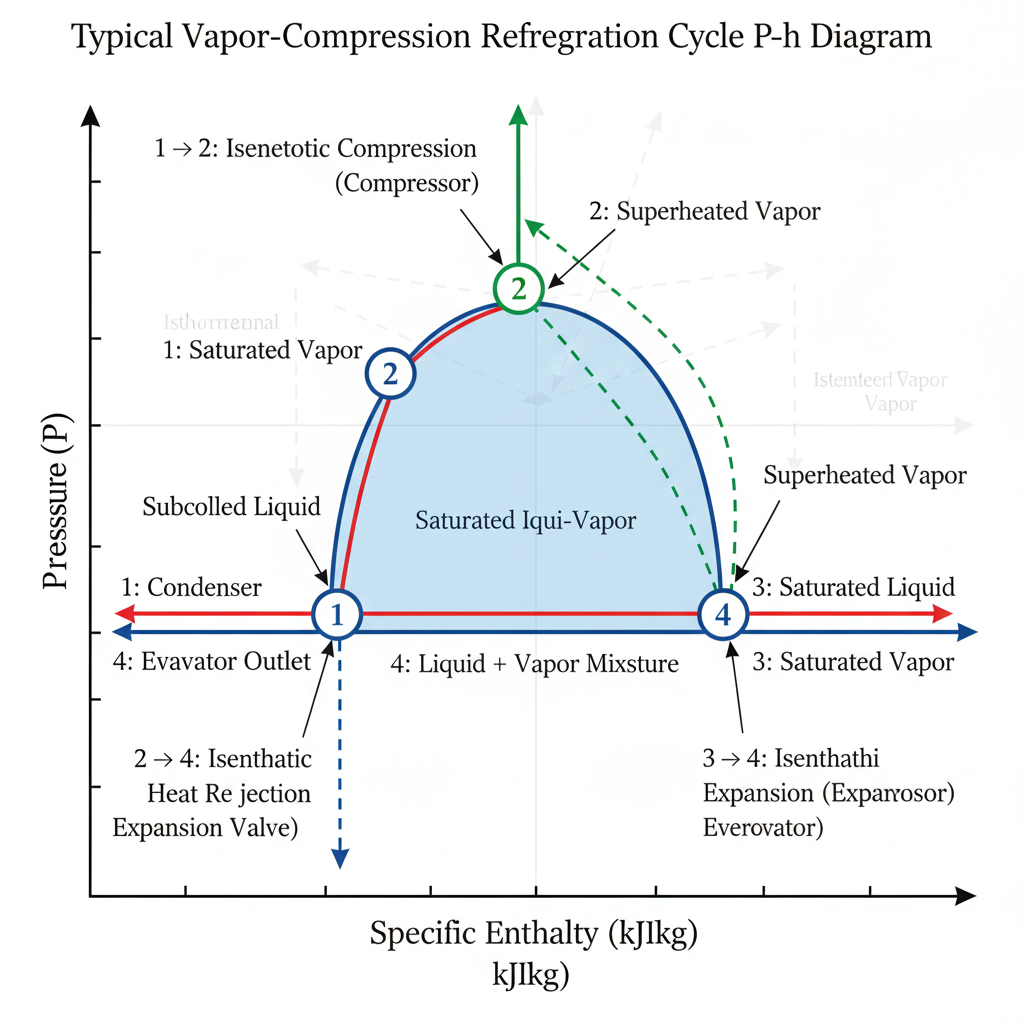
\includegraphics[width=5cm]{image copy.png}
             \caption{蒸气压缩制冷循环P-h关系}
           \end{figure}
        \end{column}
        \begin{column}{0.5\textwidth}
          \begin{itemize}
              \item \textbf{1 $\rightarrow$ 2:} 沿等熵线上升,\alert{压缩过程}。
              \item \textbf{2 $\rightarrow$ 3:} 沿等压线向左,\alert{冷凝过程}。
              \item \textbf{3 $\rightarrow$ 4:} 垂直向下,\alert{节流过程} ($h_3 = h_4$)。
              \item \textbf{4 $\rightarrow$ 1:} 沿等压线向右,\alert{蒸发过程},单位制冷量为$h_1 - h_4$。
          \end{itemize}
        \end{column}
    \end{columns}
    \vfill
    \textbf{分析:} P-h图直观地展示了节流过程作为连接高压侧和低压侧的桥梁,并为蒸发过程创造了必要的低温低压条件。
\end{frame}


\begin{frame}
  \frametitle{应用二:气体的液化}
    \begin{itemize}
    \item \textbf{基本原理:} 利用深度节流致冷,并结合\alert{回热}技术,使气体温度逐步降低到其沸点以下,从而液化。
    \vfill
    \item \textbf{林德液化循环 (Linde-Hampson Cycle):}
    \begin{itemize}
      \item \textbf{关键技术:} 结合了 \textbf{\alert{节流致冷}} 与 \textbf{\alert{回流换热}}。
      \item \textbf{流程:} 气体被压缩预冷 $\rightarrow$ 通过节流阀膨胀降温 $\rightarrow$ \alert{降温后的冷气体通过换热器去冷却后续进入的高压气体} $\rightarrow$ 反复循环,逐级降温 $\rightarrow$ 最终液化。
    \end{itemize}
    \vfill
    \item \textbf{应用实例:}
    \begin{itemize}
        \item \textbf{空气分离:} 制备液氮 ($LN_2$)、液氧 ($LO_X$)、液氩等工业气体。
        \item \textbf{能源工业:} 液化天然气 (LNG) 的生产,便于储存和长途运输。
    \end{itemize}
  \end{itemize}
\end{frame}

\begin{frame}
    \frametitle{气体液化的改进:克劳德循环}
    \begin{block}{林德循环的局限}
        完全依赖节流效应,效率相对较低,特别是对于预冷需求高的气体。
    \end{block}
    \vfill
    \begin{block}{克劳德循环 (Claude Cycle)}
        \begin{itemize}
            \item \textbf{核心改进:} 将高压气流分为两部分。一部分进入\alert{膨胀机}对外做功,产生显著的温降(近似等熵膨胀);另一部分进行传统的节流。
            \item \textbf{优势:}
            \begin{itemize}
                \item \textbf{效率更高:} 膨胀机做功产生的降温效果比单纯节流更显著。
                \item \textbf{预冷集成:} 膨胀机出来的冷气流可用于对主气路进行高效预冷。
            \end{itemize}
            \item \textbf{结论:} 现代大型气体液化装置多采用克劳德循环或其改进形式。
        \end{itemize}
    \end{block}
\end{frame}

% --- 第三部分:其他重要应用 ---
\section{其他重要应用}

\begin{frame}
  \frametitle{低温技术与工业控制}
  \begin{block}{低温技术 (Cryogenics)}
    \begin{itemize}
        \item \textbf{J-T制冷机:} 以节流过程为核心的微型制冷机,结构简单、无运动部件、振动小,可达到极低温度(液氦温区, 4K)。
        \item \textbf{应用:}
        \begin{itemize}
            \item \textbf{超导技术:} 冷却超导磁体(MRI、粒子加速器、磁悬浮)。
            \item \textbf{空间探测:} 冷却红外探测器和天文传感器,减少热噪声。
            \item \textbf{量子计算:} 为超导量子比特提供极低温环境。
        \end{itemize}
    \end{itemize}
  \end{block}
  \vfill
  \begin{block}{工业过程与能源领域}
    \begin{itemize}
        \item \textbf{动力系统:} 使用节流阀调节蒸汽流量和压力,控制汽轮机功率。
        \item \textbf{天然气处理:} 利用节流降温分离天然气中的重烃组分(NGLs)。
        \item \textbf{安全泄压:} 安全阀的快速开启可视为一个节流过程,用于保护压力容器。
    \end{itemize}
  \end{block}
\end{frame}


% --- 第四部分:总结与展望 ---
\section{总结与展望}

\begin{frame}
  \frametitle{总结}
  \begin{itemize}
    \item \textbf{物理核心:} 节流过程是\alert{等焓}过程,其应用的核心是基于实际气体分子间相互作用力的\alert{焦耳-汤姆孙效应}。
    \vfill
    \item \textbf{技术桥梁:} 它是连接热力系统中\alert{高压区}和\alert{低压区}的关键环节,是实现温降和相变的重要手段。
    \vfill
    \item \textbf{应用广度:} 从维持日常生活的\alert{冰箱空调},到支撑前沿科技的\alert{气体液化}和\alert{超导应用},节流过程是现代工业和科技中不可或缺的一环。
    \vfill
    \item \textbf{核心思想:}
    \begin{center}
        一个看似简单的物理过程,\\
        却深刻体现了从微观相互作用到宏观工程应用的转化。
    \end{center}
  \end{itemize}
\end{frame}

\begin{frame}
    \frametitle{展望}
    \begin{itemize}
        \item \textbf{新材料与工质:}
        \begin{itemize}
            \item 探索更环保、高效的新型制冷剂以应对全球变暖。
            \item 研究具有更优异J-T效应的多孔材料,用于微型制冷。
        \end{itemize}
        \vfill
        \item \textbf{集成与优化:}
        \begin{itemize}
            \item 将节流过程与其他制冷技术(如磁制冷、声制冷)相结合,开发混合式制冷循环。
            \item 利用先进的计算流体力学(CFD)优化节流元件(如膨胀阀)的结构,提高系统能效。
        \end{itemize}
        \vfill
        \item \textbf{新兴应用:}
        \begin{itemize}
            \item 在氢能源的液化、储存和运输中扮演关键角色。
            \item 在二氧化碳捕获与封存(CCS)技术中用于液化$CO_2$。
        \end{itemize}
    \end{itemize}
\end{frame}


% --- 结束页 ---
\begin{frame}
    \begin{center}
        \Huge\bfseries
         汇报结束
    \end{center}
\end{frame}


\end{document}

